\documentclass{article}
\usepackage[utf8]{inputenc}
\usepackage{geometry}
\geometry{a4paper, margin=1in}
\usepackage{amsmath}
\usepackage{amsfonts}
\usepackage{amssymb}
\usepackage{graphicx}
\usepackage{enumitem}
\usepackage{xcolor}
\usepackage{tikz}
\usetikzlibrary{shapes.geometric, arrows.meta, positioning}

\title{Project-X: Agent-Based Architecture Module Descriptions}
\author{}
\date{July 18, 2025}

\begin{document}
\maketitle

This document describes the modules of the new agent-based architecture for Project-X, leveraging Ollama for LLM capabilities and LangGraph for agent orchestration, updated as of 06:57 AM CST. The architecture is designed to support multiple use cases, such as fraud detection, supply chain optimisation, and customer analytics, ensuring flexibility and scalability.

\section{Core Technologies}
\begin{itemize}
    \item \textbf{Ollama:} Serves as the local Large Language Model (LLM) provider for all agents, ensuring privacy, cost-effectiveness, and control over the specific models utilised.
    \item \textbf{LangGraph:} The primary framework for orchestrating complex, stateful multi-agent workflows, particularly central to the Decision Engine.
    \item \textbf{Existing Tools:} Continued reliance on established systems like Kafka, DIVIDL, existing Machine Learning (ML) APIs, and Business Rules Services, which serve as ``tools'' for the agents to interact with.
\end{itemize}

\section{Modules}

\subsection{Data Sources}
\begin{itemize}
    \item \textbf{SAPI Oracle ERP:} Enterprise Resource Planning system, providing core business data.
    \item \textbf{Salesforce:} Customer Relationship Management (CRM) platform, source of sales and customer data.
    \item \textbf{Operational Systems:} Various other systems providing data from daily operations.
    \item \textbf{Custom Solutions/DBs:} Bespoke databases or applications for specialised data.
\end{itemize}

\subsection{Data Ingestion \& Initial Processing (Agent-Enhanced)}
This layer combines traditional data streaming with intelligent, agent-driven processing.
\begin{itemize}
    \item \textbf{Connectors (React to business events):} Interface directly with source systems to ingest data in real-time or near real-time (planned for post-MVP integration).
    \item \textbf{Kafka:} Distributed streaming platform for high-throughput, low-latency data ingestion.
    \item \textbf{DIVIDL:} A data lake or initial processing component for storing raw and semi-processed data.
    \item \textbf{Data Ingestion Agents (Stream Processor Agent):}
        \begin{itemize}
            \item \textbf{Role:} Monitor Kafka topics and DIVIDL for new data streams (initially synthetic data).
            \item \textbf{Capabilities:} Utilises Ollama LLMs for intelligent parsing, hybrid validation (combining strict rules with semantic understanding), dynamic data routing based on content, rich metadata generation, and data summarisation for monitoring.
            \item \textbf{Tools:} Kafka API/client libraries, DIVIDL APIs, database connectors, data validation libraries, data profiling tools.
        \end{itemize}
    \item \textbf{Synthetic Data Generation Agent (Code Generator):}
        \begin{itemize}
            \item \textbf{Role:} Generates synthetic data (tabular or time series) for MVP testing/development across various use cases.
            \item \textbf{Capabilities:} Interprets natural language dataset descriptions and generates executable Python code (e.g., using Faker or SciPy) to produce realistic synthetic datasets. The LLM generates code, external processes execute it.
            \item \textbf{Tools:} Access to a code execution environment, data generation libraries (Faker, SciPy).
        \end{itemize}
    \item \textbf{Raw Gold Data / Source Gold Bronze Data:} Data zones representing raw and initially curated data.
    \item \textbf{Validation Strategy:}
        \begin{itemize}
            \item \textbf{Synthetic Data Validation:} Statistical tests (e.g., Kolmogorov-Smirnov, Chi-Square) ensure synthetic data aligns with use case-specific distributions (e.g., financial transactions, customer interactions). Tools: SciPy, pandas. Success metric: p-value > 0.05.
            \item \textbf{Code Validation:} Generated Python code is tested using pytest with predefined test cases covering diverse use case scenarios. Success metric: 95\% test case pass rate, no runtime errors. Human review ensures code efficiency.
            \item \textbf{Data Ingestion Validation:} Hybrid validation combines rule-based checks with LLM-driven semantic validation to ensure data integrity across domains. Success metric: 98\% accuracy in routing and metadata generation.
        \end{itemize}
    \item \textbf{Performance Testing:}
        \begin{itemize}
            \item \textbf{Scenarios:} Stress-test Kafka ingestion with high-throughput data streams (e.g., 1000 events/second for customer analytics, 500 transactions/second for fraud detection). Simulate LLM-driven parsing under load.
            \item \textbf{Tools:} Apache JMeter for load testing Kafka, Locust for API testing, Prometheus for monitoring CPU/memory usage.
            \item \textbf{Metrics:} Latency < 100ms for data routing, throughput > 1000 events/second, resource utilisation < 80\%.
            \item \textbf{Mitigation:} Implement caching for LLM queries and parallel processing for data streams to optimise performance.
        \end{itemize}
    \item \textbf{Integration Strategy:}
        \begin{itemize}
            \item \textbf{Real-Time Integration (Post-MVP):} Connectors interface with Data Sources (e.g., SAPI Oracle ERP, Salesforce) to stream data into Kafka topics, processed by Data Ingestion Agents and stored in DIVIDL for use case-specific workflows.
            \item \textbf{Error Handling:} Implement exponential backoff retries for failed Kafka consumer requests, dead-letter queues for unprocessable events, and logging (e.g., Log4j) for error tracking.
            \item \textbf{Latency Optimisation:} Use batch processing for high-throughput streams and parallel processing for LLM-driven tasks to minimise latency.
            \item \textbf{Tools:} Kafka Streams API, DIVIDL APIs, Log4j for logging, Prometheus for monitoring.
            \item \textbf{Metrics:} Ingestion latency < 50ms, error rate < 1\%, successful event processing > 99\%.
        \end{itemize}
\end{itemize}

\subsection{Predictive Engine (AutoML Agent)}
Focuses on dynamic machine learning model creation and serving.
\begin{itemize}
    \item \textbf{ML Repository:} Stores machine learning models, algorithms, and training data.
    \item \textbf{ML as an API:} Provides endpoints for serving trained ML models for inference.
    \item \textbf{AutoML Orchestration Agent:}
        \begin{itemize}
            \item \textbf{Role:} Given a synthetic dataset and a task (prediction/classification), it intelligently proposes and generates ML model pipelines for various use cases.
            \item \textbf{Capabilities:} Utilises Ollama LLMs to analyse data, understand task requirements, and generate PyCaret code for data pre-processing, feature engineering, model selection, hyperparameter tuning, and evaluation.
            \item \textbf{Tools:} PyCaret library, data analysis libraries, existing ML as an API, database access for training data.
        \end{itemize}
    \item \textbf{Validation Strategy:}
        \begin{itemize}
            \item \textbf{Pipeline Validation:} Generated ML pipelines are evaluated using cross-validation and performance metrics (e.g., F1-score, AUC) tailored to use case requirements. Tools: PyCaret, scikit-learn. Success metric: Model performance meets use case-specific thresholds (e.g., F1 > 0.85 for classification).
            \item \textbf{Human Review:} Domain experts review pipeline configurations for relevance to specific use cases.
        \end{itemize}
\end{itemize}

\subsection{Precision Engine (Natural Language Rules Agent)}
Manages and applies business rules with enhanced flexibility via LLMs.
\begin{itemize}
    \item \textbf{Business Rules Config Service:} Manages the definition and storage of business rules.
    \item \textbf{Business Rules Execution Service:} Executes defined business rules.
    \item \textbf{Business Rule Management Agent:}
        \begin{itemize}
            \item \textbf{Role:} Facilitates intuitive creation, modification, and intelligent application of business rules.
            \item \textbf{Capabilities:} Uses Ollama LLMs to interpret natural language rule descriptions from the UI, translating them into structured formats.
            \item \textbf{Tools:} APIs to Business Rules Config Service and Business Rules Execution Service.
        \end{itemize}
    \item \textbf{Validation Strategy:}
        \begin{itemize}
            \item \textbf{Rule Translation Validation:} LLM-translated rules are cross-checked against a test suite of known scenarios for multiple use cases. Tools: Custom validation scripts, Business Rules Execution Service API. Success metric: 98\% accuracy in translation.
            \item \textbf{Human Review:} Business analysts verify rule translations for intent and correctness across domains.
        \end{itemize}
\end{itemize}

\subsection{Decision Engine (LangGraph Core)}
The central intelligent hub for complex, adaptive decision-making, powered by LangGraph.
\begin{itemize}
    \item \textbf{LangGraph-Powered Orchestration:} The core of this module, where the decision workflow is defined as a dynamic, stateful graph of interacting agents.
    \item \textbf{Decision Orchestration Supervisor Agent (LangGraph Graph):}
        \begin{itemize}
            \item \textbf{Role:} The primary controller of the decision process. It dynamically determines the sequence of actions, manages context, handles collaboration between sub-agents, and generates explanations for decisions.
            \item \textbf{Capabilities:} Adaptive workflow execution, contextual reasoning, inter-agent collaboration, explanation generation, and uncertainty handling (e.g., routing to Human-in-the-Loop).
        \end{itemize}
    \item \textbf{Sub-Agents (Nodes within the LangGraph):}
        \begin{itemize}
            \item \textbf{Prediction Request Agent:} Interacts with the ML as an API to retrieve predictions.
            \item \textbf{Rule Application Agent:} Calls the Business Rules Execution Service to apply business logic.
            \item \textbf{Data Query Agent:} Accesses internal databases or external APIs for additional contextual information.
            \item \textbf{Human-in-the-Loop Agent:} Facilitates human intervention for review, approval, or override of decisions.
            \item \textbf{Conflict Resolution Agent:} Identifies and attempts to reconcile conflicting information between ML predictions and business rules.
        \end{itemize}
    \item \textbf{Tools for Decision Engine Agents:} APIs to ML as an API, Business Rules Execution Service, internal databases, external APIs, logging/auditing services.
    \item \textbf{Validation Strategy:}
        \begin{itemize}
            \item \textbf{Explanation Validation:} Decision explanations are evaluated for clarity and completeness using a predefined rubric. Tools: Logging/auditing services, custom evaluation scripts. Success metric: 90\% of explanations rated as ``clear'' by human reviewers; no critical logical errors.
            \item \textbf{Conflict Resolution Validation:} Conflicts are logged and reviewed to ensure resolution logic aligns with use case goals. Success metric: 95\% of conflicts resolved without human intervention.
        \end{itemize}
    \item \textbf{Performance Testing:}
        \begin{itemize}
            \item \textbf{Scenarios:} Stress-test LangGraph workflows with complex decision paths (e.g., 100 concurrent decisions for supply chain optimisation). Simulate LLM inference under high load.
            \item \textbf{Tools:} Locust for API testing, Prometheus for monitoring, custom scripts for workflow benchmarking.
            \item \textbf{Metrics:} Decision latency < 100ms, throughput > 100 decisions/second, resource utilisation < 80\%.
            \item \textbf{Mitigation:} Use load balancing for LangGraph nodes and caching for repetitive LLM queries to optimise performance.
        \end{itemize}
\end{itemize}

\subsection{Orchestrator}
\begin{itemize}
    \item \textbf{Role:} Acts as the primary API gateway, routing user requests from the UI to the appropriate entry points within the LangGraph-powered Decision Engine and translating responses back to the UI.
    \item \textbf{Functionality:} Handles communication between the frontend and the agentic backend, with much of the complex workflow logic now residing within LangGraph.
\end{itemize}

\subsection{User Interface (UI)}
Provides a comprehensive interface for user interaction and system management.
\begin{itemize}
    \item \textbf{Simulation Configuration:} Allows users to define and run decision scenarios.
    \item \textbf{Define Business Rules:} Users can define rules using natural language, interpreted by the Business Rule Management Agent.
    \item \textbf{Define Workflow (Visual LangGraph Editor):} Enables users to visually design, modify, and monitor the LangGraph workflows for the Decision Engine (planned for post-MVP).
    \item \textbf{Simulate by Changing Variables:} Allows for testing decision logic with varied inputs, enhanced by step-by-step agent reasoning explanations.
    \item \textbf{User Journey Definition:} For defining and simulating end-to-end user processes that interact with the agent system.
    \item \textbf{Agent Interaction Interface:} A new feature for monitoring agent activity, reviewing explanations for decisions, and providing human input or overrides (basic version for MVP).
\end{itemize}

\subsection{Validation Architecture}
\begin{figure}[h]
    \centering
    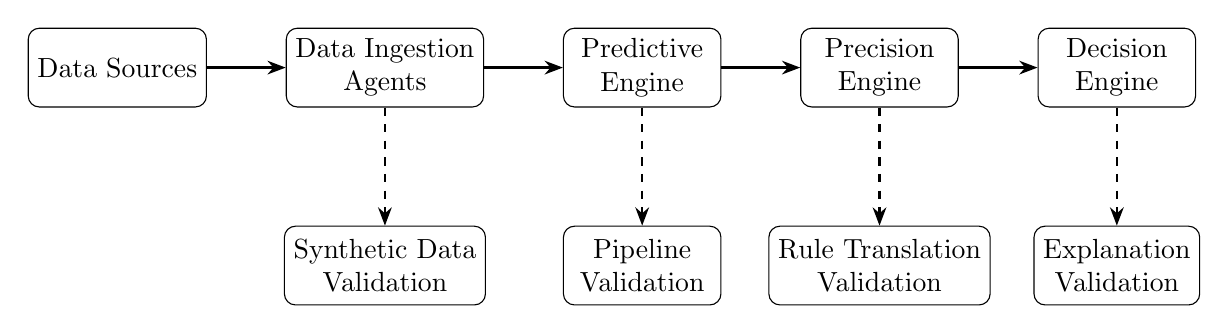
\begin{tikzpicture}[
        node distance=1.5cm and 1cm,
        box/.style={rectangle, draw, rounded corners, minimum height=1cm, minimum width=2cm, align=center},
        arrow/.style={-Stealth, thick}
    ]
        % Nodes
        \node[box] (data) {Data Sources};
        \node[box, right=of data] (ingestion) {Data Ingestion\\Agents};
        \node[box, right=of ingestion] (predictive) {Predictive\\Engine};
        \node[box, right=of predictive] (precision) {Precision\\Engine};
        \node[box, right=of precision] (decision) {Decision\\Engine};
        \node[box, below=of ingestion] (validation1) {Synthetic Data\\Validation};
        \node[box, below=of predictive] (validation2) {Pipeline\\Validation};
        \node[box, below=of precision] (validation3) {Rule Translation\\Validation};
        \node[box, below=of decision] (validation4) {Explanation\\Validation};

        % Arrows
        \draw[arrow] (data) -- (ingestion);
        \draw[arrow] (ingestion) -- (predictive);
        \draw[arrow] (predictive) -- (precision);
        \draw[arrow] (precision) -- (decision);
        \draw[arrow, dashed] (ingestion) -- (validation1);
        \draw[arrow, dashed] (predictive) -- (validation2);
        \draw[arrow, dashed] (precision) -- (validation3);
        \draw[arrow, dashed] (decision) -- (validation4);
    \end{tikzpicture}
    \caption{Validation Architecture for Project-X}
    \label{fig:validation_architecture}
\end{figure}

\subsection{Performance Testing Architecture}
\begin{figure}[h]
    \centering
    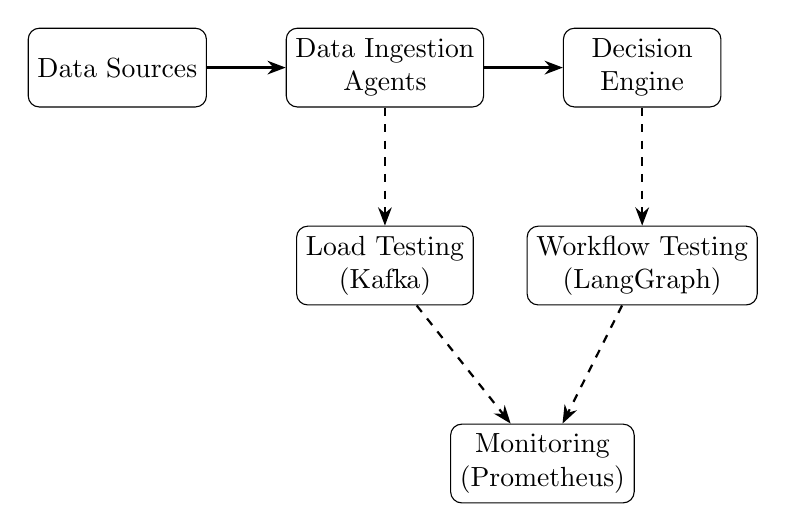
\begin{tikzpicture}[
        node distance=1.5cm and 1cm,
        box/.style={rectangle, draw, rounded corners, minimum height=1cm, minimum width=2cm, align=center},
        arrow/.style={-Stealth, thick}
    ]
        % Nodes
        \node[box] (data) {Data Sources};
        \node[box, right=of data] (ingestion) {Data Ingestion\\Agents};
        \node[box, right=of ingestion] (decision) {Decision\\Engine};
        \node[box, below=of ingestion] (test1) {Load Testing\\(Kafka)};
        \node[box, below=of decision] (test2) {Workflow Testing\\(LangGraph)};
        \node[box, below=of test1, xshift=2cm] (monitor) {Monitoring\\(Prometheus)};

        % Arrows
        \draw[arrow] (data) -- (ingestion);
        \draw[arrow] (ingestion) -- (decision);
        \draw[arrow, dashed] (ingestion) -- (test1);
        \draw[arrow, dashed] (decision) -- (test2);
        \draw[arrow, dashed] (test1) -- (monitor);
        \draw[arrow, dashed] (test2) -- (monitor);
    \end{tikzpicture}
    \caption{Performance Testing Architecture for Project-X}
    \label{fig:performance_architecture}
\end{figure}

\subsection{Integration Architecture}
\begin{figure}[h]
    \centering
    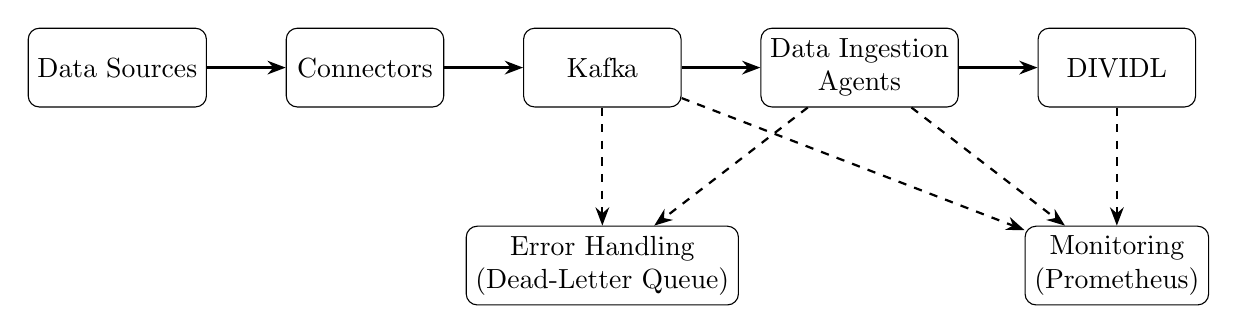
\begin{tikzpicture}[
        node distance=1.5cm and 1cm,
        box/.style={rectangle, draw, rounded corners, minimum height=1cm, minimum width=2cm, align=center},
        arrow/.style={-Stealth, thick}
    ]
        % Nodes
        \node[box] (data) {Data Sources};
        \node[box, right=of data] (connectors) {Connectors};
        \node[box, right=of connectors] (kafka) {Kafka};
        \node[box, right=of kafka] (ingestion) {Data Ingestion\\Agents};
        \node[box, right=of ingestion] (dividl) {DIVIDL};
        \node[box, below=of kafka] (error) {Error Handling\\(Dead-Letter Queue)};
        \node[box, below=of dividl] (monitor) {Monitoring\\(Prometheus)};

        % Arrows
        \draw[arrow] (data) -- (connectors);
        \draw[arrow] (connectors) -- (kafka);
        \draw[arrow] (kafka) -- (ingestion);
        \draw[arrow] (ingestion) -- (dividl);
        \draw[arrow, dashed] (kafka) -- (error);
        \draw[arrow, dashed] (ingestion) -- (error);
        \draw[arrow, dashed] (kafka) -- (monitor);
        \draw[arrow, dashed] (ingestion) -- (monitor);
        \draw[arrow, dashed] (dividl) -- (monitor);
    \end{tikzpicture}
    \caption{Integration Architecture for Project-X}
    \label{fig:integration_architecture}
\end{figure}

\subsection{Global Architecture}
\begin{figure}[h]
    \centering
    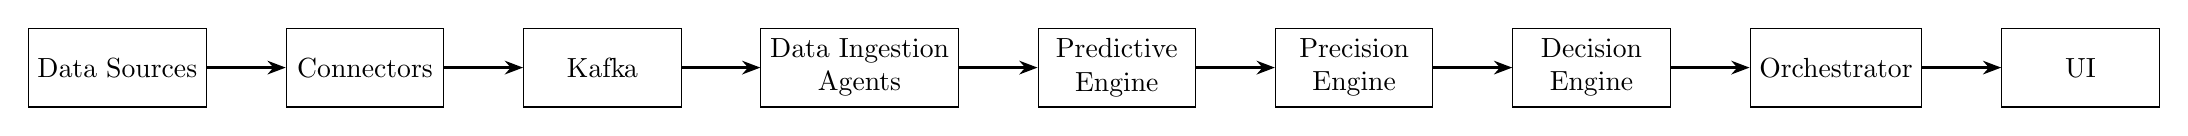
\begin{tikzpicture}[
        node distance=1.5cm and 1cm,
        box/.style={rectangle, draw, minimum height=1cm, minimum width=2cm, align=center},
        arrow/.style={-Stealth, thick}
    ]
        % Nodes
        \node[box] (data) {Data Sources};
        \node[box, right=of data] (connectors) {Connectors};
        \node[box, right=of connectors] (kafka) {Kafka};
        \node[box, right=of kafka] (ingestion) {Data Ingestion\\Agents};
        \node[box, right=of ingestion] (predictive) {Predictive\\Engine};
        \node[box, right=of predictive] (precision) {Precision\\Engine};
        \node[box, right=of precision] (decision) {Decision\\Engine};
        \node[box, right=of decision] (orchestrator) {Orchestrator};
        \node[box, right=of orchestrator] (ui) {UI};

        % Arrows
        \draw[arrow] (data) -- (connectors);
        \draw[arrow] (connectors) -- (kafka);
        \draw[arrow] (kafka) -- (ingestion);
        \draw[arrow] (ingestion) -- (predictive);
        \draw[arrow] (predictive) -- (precision);
        \draw[arrow] (precision) -- (decision);
        \draw[arrow] (decision) -- (orchestrator);
        \draw[arrow] (orchestrator) -- (ui);
    \end{tikzpicture}
    \caption{Global Architecture of the New Agent-Based System}
    \label{fig:global_architecture}
\end{figure}

\end{document}